\chapter{実装の方針} \label{implementation}

フロントエンドに lively.next\footnote{\url{https://lively-next.org}} を、方程式の処理と数値計算に SymPy~\cite{meurer_sympy_2017} を用い、JavaScript と Python を組み合わせて実装する。また、 Pyodide~\footnote{\url{https://pyodide.org/en/stable/}} を用いることで、ブラウザ上で全ての計算を行う。
% lively.next は、GUIアプリケーションを作成・実行するためのWebプログラミング環境である。学習者が物体や方程式を定義する画面とシミュレーションを表示する画面を lively.next で作成する。SymPy は、記号計算のための Python ライブラリであり、Pyodide~\footnote{\tiny{\url{https://github.com/pyodide/pyodide}}} を用いることで WebAssembly に変換し、ブラウザで実行する。\simname は、入力された物理量や方程式を SymPy オブジェクトに変換することで、数値計算を可能にする。シミュレーションの実行時は、設定された時刻 $t$ の範囲を粒度 $\Delta t$ ずつ変化させる。各方程式に各 $t$ を代入した結果を lively.next が受け取り、描画する。シミュレーションのリアルタイム性を確保するため、各 $t$ を方程式に代入した値は方程式の定義時・変数の値の変更時にあらかじめ計算する。

\section{lively.next}
lively.next は Lively~\cite{ingalls_2008}から派生したプロジェクトで、ブラウザ上で GUI アプリケーションを作成・実行することができる Web プログラミング環境である。これを用いて、学習者が物体や方程式を定義する物理系定義ペインと、シミュレーション結果を表示する観測ペインを実装する。ブラウザ上で利用できるため、学習者はソフトウェアのインストールなどをする必要がなく、簡単に利用できる。

\begin{figure}[hbt]
\centering
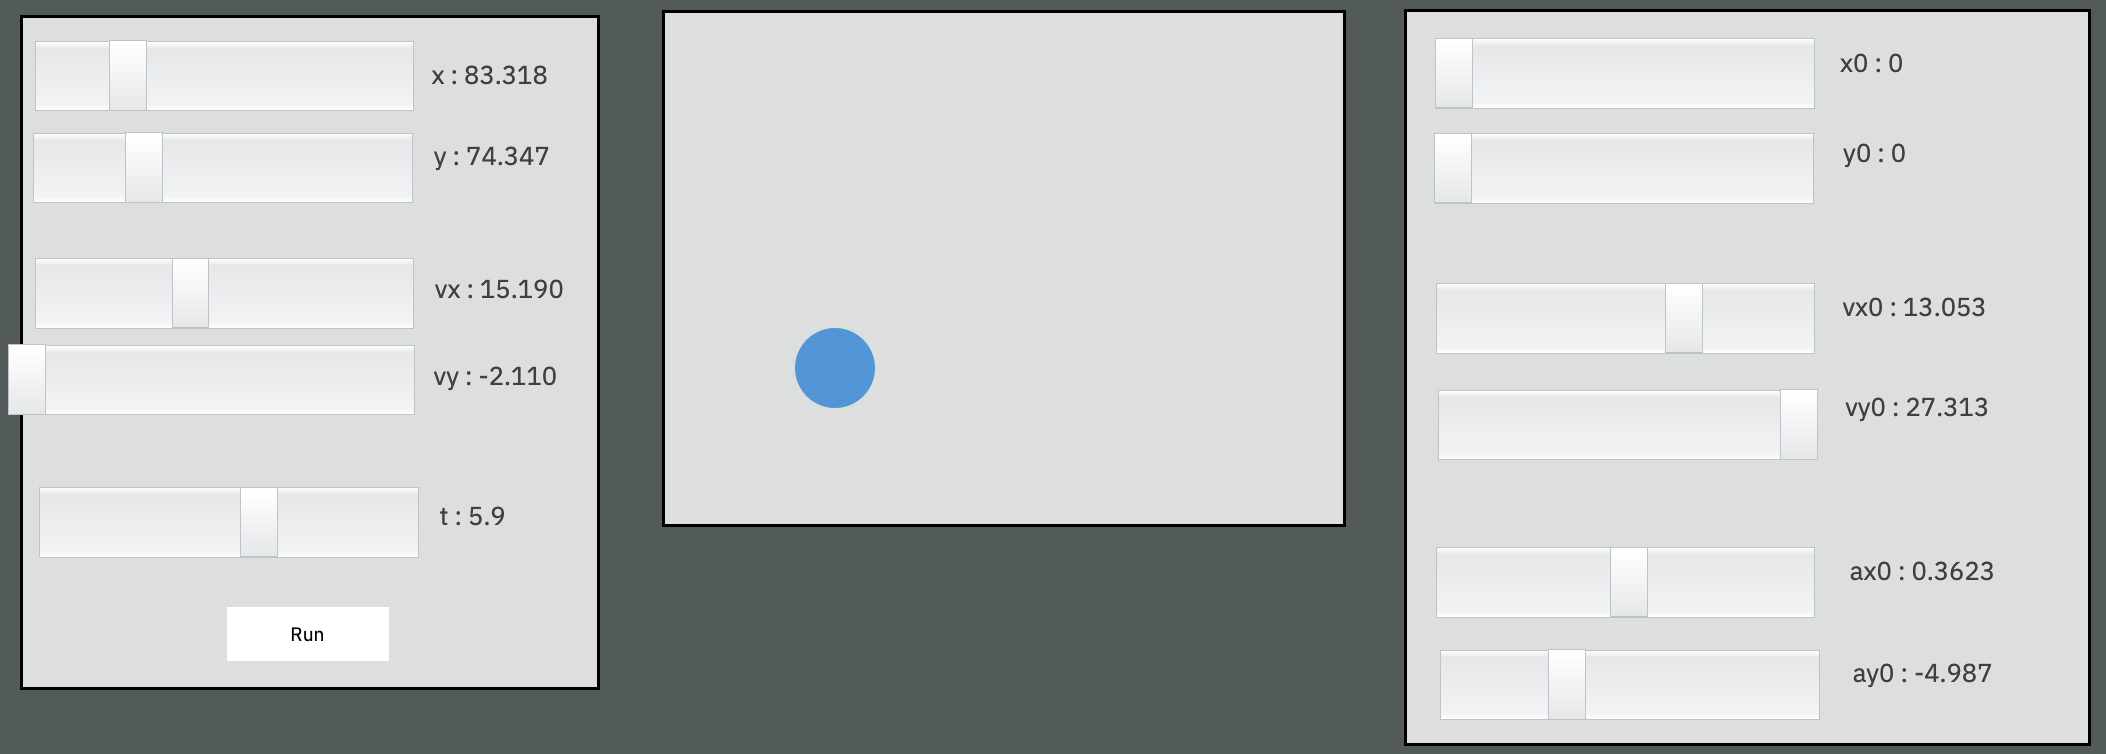
\includegraphics[width=0.9\linewidth]{figure/lively_example.png}
\caption{lively.next を用いて実装されたシミュレーション結果の表示画面}
\end{figure}

\section{SymPy}
SymPy は、記号計算のための Python ライブラリである。次元付き変数を作成し、方程式の処理や数値計算を行うことができる。図~\ref{sympy_example}は、実際に SymPy で斜方投射を表す物理系を定義する例である。

\begin{figure}[p]
\centering
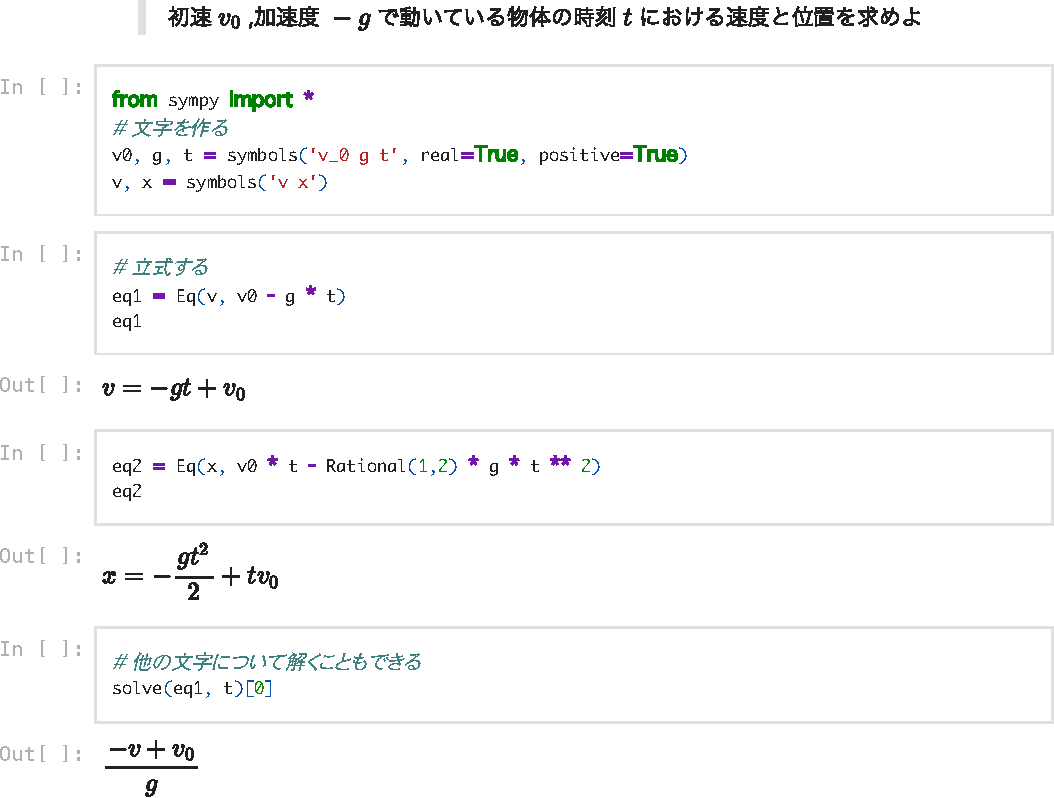
\includegraphics[width=\linewidth]{work/SymPy_example-crop.pdf}
\caption{SymPy を用いて斜方投射を表す物理系を定義する例} \label{sympy_example}
\end{figure}

SymPy は次元を扱うことはできるのだが、次元が異なる値同士も足すことができてしまう。図~\ref{sympy_unit_example}では、$t$ に次元 $\mathrm{[T]}$ を、$g$ に次元 $\mathrm{[T/S^2]}$ を割り当てたが、$t + g$ が計算できてしまう。そのため、このような不一致を検出する仕組みを実装する必要がある。

\begin{figure}[t]
\centering
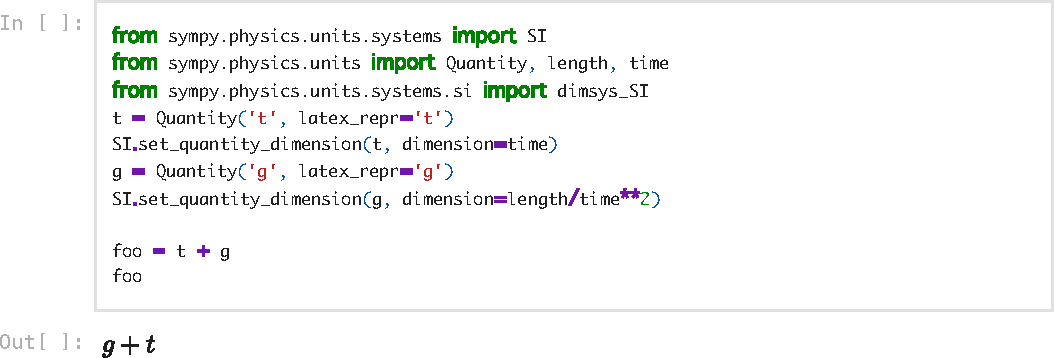
\includegraphics[width=\linewidth]{work/sympy_unit_example-crop.pdf}
\caption{SymPy 上で単位が異なる値同士を足す例} \label{sympy_unit_example}
\end{figure}

また、SymPy は Python のライブラリであるが、後述する Pyodide を用いることでブラウザ上で実行することができる。

\section{Pyodide}
Pyodide は、Mozilla が開発している WebAssembly で実装された CPython 処理系である。ブラウザ上でピュアな Python コードを実行できる。また、Python で書かれたパッケージと C 言語で書かれた一部のパッケージに対応していて、SymPy は Pyodide で実行可能である。実際に Pyodide を実行する例を図~\ref{pyodide_example}に記す。

\begin{figure}[h]
\centering
\begin{lstlisting}[language=html]
<!DOCTYPE html>
<head>
  <script src="https://cdn.jsdelivr.net/pyodide/v0.22.0/full/pyodide.js"></script>
  <script>
    async function main() {
      let pyodide = await loadPyodide();
      let result = pyodide.runPython(`
import js
result_div = js.document.getElementById("result")
x = 2
y = 10
result_div.textContent = x ** y
      `);
    }
  </script>
</head>
<body>
  <script>main()</script>
  <p>結果</p>
  <p id="result" style="float: left"></p>
</body>
\end{lstlisting}
% \includegraphics*[width=0.1\linewidth]{work/pyodide_example.png}
\caption{Pyodide を利用する例} \label{pyodide_example}
\end{figure}

% 結果を KaTeX を用いて表示した例を図\ref{Pyodide_result}に記す。

% \newgeometry{left=1cm, right=1cm}
% \begin{figure}[htb]
% \begin{lstlisting}[language=html]
% <!DOCTYPE html>
% <head>
%   <script src="https://cdn.jsdelivr.net/pyodide/v0.22.0/full/pyodide.js"></script>
%   <link rel="stylesheet" href="https://cdn.jsdelivr.net/npm/katex@0.16.4/dist/katex.min.css" integrity="sha384-vKruj+a13U8yHIkAyGgK1J3ArTLzrFGBbBc0tDp4ad/EyewESeXE/Iv67Aj8gKZ0" crossorigin="anonymous">
%   <script defer src="https://cdn.jsdelivr.net/npm/katex@0.16.4/dist/katex.min.js" integrity="sha384-PwRUT/YqbnEjkZO0zZxNqcxACrXe+j766U2amXcgMg5457rve2Y7I6ZJSm2A0mS4" crossorigin="anonymous"></script>
%   <script defer src="https://cdn.jsdelivr.net/npm/katex@0.16.4/dist/contrib/auto-render.min.js" integrity="sha384-+VBxd3r6XgURycqtZ117nYw44OOcIax56Z4dCRWbxyPt0Koah1uHoK0o4+/RRE05" crossorigin="anonymous" onload="renderMathInElement(document.body);"></script>
% </head>
% <body>
%   <script>
%     async function main() {
%       let pyodide = await loadPyodide();
%       await pyodide.loadPackage("sympy");
%       let code = `
%       from sympy import symbols, Eq, solve, latex
%       v0, g, t = symbols('v_0 g t', real=True, positive=True)
%       v = symbols('v')
%       eq1 = Eq(v, v0 - g * t)
%       latex(solve(eq1, t)[0])
%       `;
%       let result = pyodide.runPython(code);
%       let resultDiv = document.getElementById("result");
%       resultDiv.textContent = `\\[${result}\\]`;
%       renderMathInElement(resultDiv);
%     };
%     main();
%   </script>
%   <p>結果</p><div id="result" style="float: left"></div>
% </body>
% \end{lstlisting}
% \caption{Pyodide を実行する例} \label{Pyodide_example}
% \end{figure}
% \restoregeometry

% \begin{figure}[htb]
% \centering
% 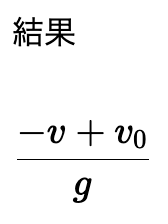
\includegraphics{work/pyodide_screenshot.png}
% \caption{実行結果} \label{Pyodide_result}
% \end{figure}
